\documentclass[12pt,a4paper]{article}
\usepackage[slovene]{babel}
\usepackage{amsmath}
\usepackage{amsfonts}
\usepackage{amssymb}
\usepackage{graphicx}
\usepackage{lmodern}
\usepackage{hyperref}
\usepackage{xcolor}

\usepackage[left=2cm,right=2cm,top=2cm,bottom=2cm]{geometry}
\author{Tina Zwittnig 64200432}
\title{Poročilo 9. vaje pri predmetu OVS \\ Geometrijska poravnava slik}

\begin{document}
\maketitle
\pagebreak
\section{computeError}
\begin{verbatim}
function [R2, MSE] = computeError(rCP, iCP, oCP, rImage, iImage, oImage, iArea)
%computeError izračuna izračuna povprečno kvadratno razdaljo med vsemi pari
%kontrolnih točk in srednjo napako sivinjskih vrednosti slike. 

T = rCP - iCP;
R11 = mean(T(1).^2+T(2).^2);
T2 = oCP - rCP;
R22 = mean(T2(1).^2+T2(2).^2);
R2 = [R11 R22];
x0 = iArea(1);
y0 = iArea(2);
w = iArea(3);
h = iArea(4);
if x0>0 && y0>0
    MSE1 = mean(mean((rImage(y0:y0+h,x0:x0+w)-iImage(y0:y0+h,x0:x0+w)).^2));
    MSE2 = mean(mean((oImage(y0:y0+h,x0:x0+w)-rImage(y0:y0+h,x0:x0+w)).^2));
    MSE = [MSE1 MSE2];
end
end
\end{verbatim}
\section{Uporabniški vmesnik}
\begin{figure}[h!]
  \begin{center}
    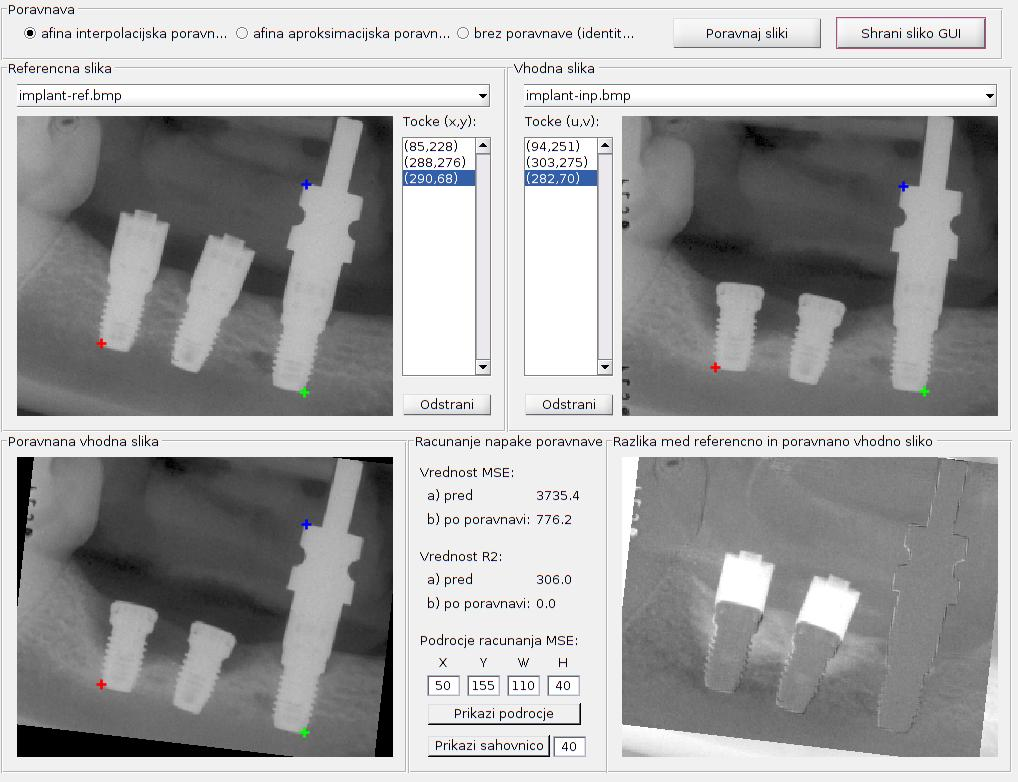
\includegraphics[scale = 0.4]{GUI1.jpg}
    \caption{Afina interpolacijska poravnava. }
    \label{fig:}
  \end{center}
\end{figure}
Kot lahko vidimo je R2 po poravnavi 0, kar je logično saj kontrolne točke preslikamo v referenčne kontrolne točke.
\begin{figure}[h!]
  \begin{center}
    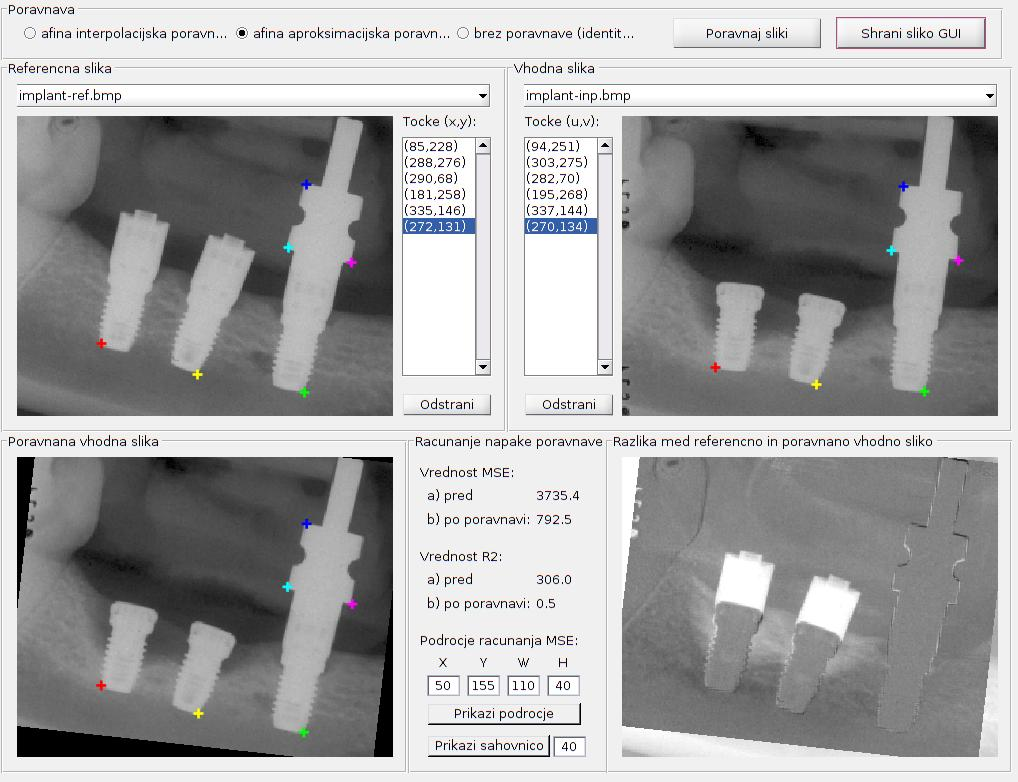
\includegraphics[scale = 0.35]{GUI2.jpg}
    \caption{Afina aproksimacijska poravnava z šestimi točkami. }
    \label{fig:}
  \end{center}
\end{figure}
\begin{figure}[h!]
  \begin{center}
    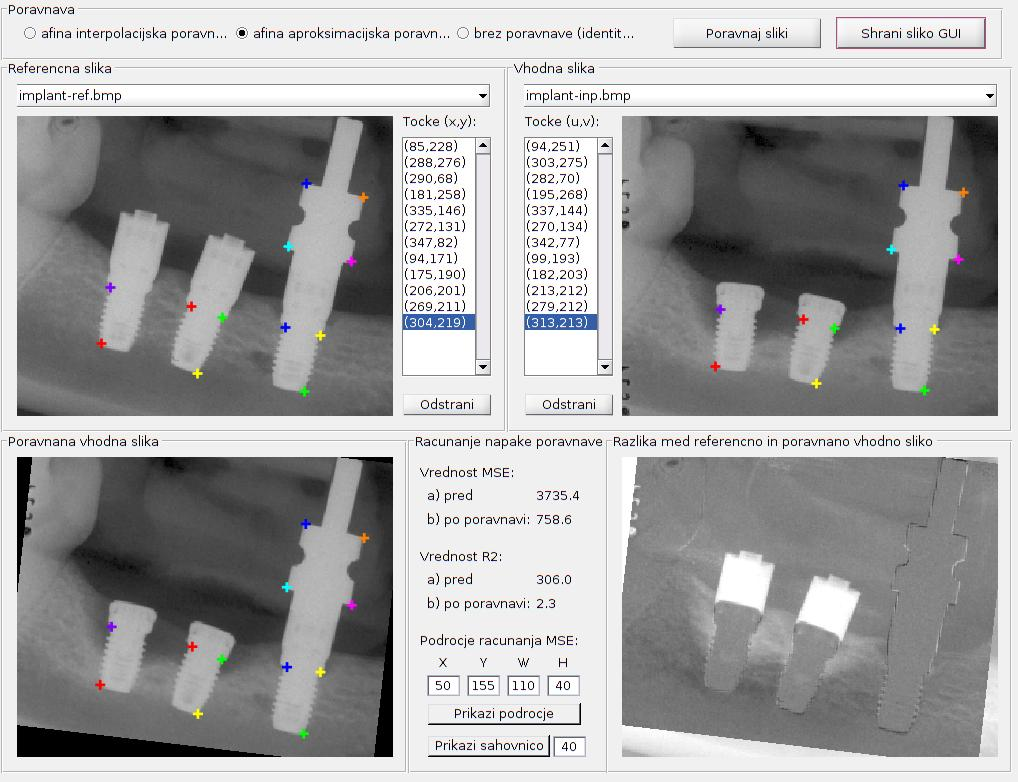
\includegraphics[scale = 0.35]{GUI3.jpg}
    \caption{Afina aproksimacijska poravnava z dvanajstimi točkami. }
    \label{fig:}
  \end{center}
\end{figure}
\section{Izčrpno iskanje največje podobnosti}
\begin{figure}[h!]
  \begin{center}
    \includegraphics[scale = 0.3]{premik1.png}
    \caption{referenčna slika, vhodna slika, premaknjena slika za optimalne parametre}
    \label{fig:}
  \end{center}
\end{figure}
Optimalni parametri za prvo vhodno sliko so x = -7mm y = 5mm. \\
\begin{figure}[h!]
  \begin{center}
    \includegraphics[scale = 0.8]{sivinske1.png}
    \caption{Izris porazdelitve izračunane mere podobnosti v prostoru premikov}
    \label{fig:}
  \end{center}
\end{figure}
\pagebreak
\begin{figure}[h!]
  \begin{center}
    \includegraphics[scale = 0.3]{premik2.png}
    \caption{referenčna slika, vhodna slika, premaknjena slika za optimalne parametre}
    \label{fig:}
  \end{center}
\end{figure} 
\begin{figure}[h!]
  \begin{center}
    \includegraphics[scale = 0.8]{sivinske2.png}
    \caption{Izris porazdelitve izračunane mere podobnosti v prostoru premikov}
    \label{fig:}
  \end{center}
\end{figure}

Optimalni parametri za drugo vhodno sliko so x = 9mm y = -3mm.
\end{document}
